\chapter[Metodologia]{Metodologia}

Este capítulo descreve todas as etapas da metodologia aplicada na elaboração deste trabalho. Primeiramente, há a classificação da \nameref{pc}, conhecendo a sua natureza de pesquisa, objetivos e procedimentos. Após, a \nameref{mpi} onde é explicado as das técnicas de pesquisa bibliográfica aplicadas. Na seção de \nameref{md} é exemplificado cada atividade e processo seguido na elaboração do trabalho. A \nameref{mar} descreve de forma sucinta o plano para análise e divulgação de resultados. Já o \nameref{fa} objetivamente demonstra a orientação por etapas para desenvolvimento do trabalho e o fluxo geral de atividades que compreende os Trabalhos de Conclusão de Curso 1 e 2. Por fim, é apresentado o \nameref{crono} de atividades e as \nameref{considfinal} do capítulo.

\section{Pesquisa Cientifica}
\label{pc}
Pesquisa pode ser definida como o procedimento racional e sistemático que tem como objetivo proporcionar respostas aos problemas que são propostos. \cite{metodologia2}.

Segundo \cite{metodologia1} "A pesquisa científica é o resultado de um inquérito ou examen minucioso realizado com o objetivo de resolver um problema, recorrendo a procedimentos científicos". Desta forma, a pesquisa pode ser classificada de acordo com diversos tipos. Quanto a \textbf{abordagem}, a pesquisa pode ser classificada como qualitativa ou quantitativa. Quanto a \textbf{natureza} pode ser classificada como uma pesquisa básica, ou aplicada. Quanto aos \textbf{objetivos} temos a pesquisa: exploratória, descritiva ou explicativa. Por fim, quanto aos \textbf{procedimentos} a pesquisa pode ser classificada como: experimental, bibliográfica, documental, de campo, ex-post-facto, de levantamento, como \textit{survey}, estudo de caso, participante, pesquisa-ação, etnográfica ou etnometodológica.

\subsection{Abordagem}

A pesquisa quantitativa, tem como foco o pensamento lógico, onde é enfatizado o raciocínio dedutivo, as regras lógicas e os atributos mensuráveis, enquanto a pesquisa qualitativa, procura evidenciar aspectos dinâmicos, holísticos e individuais, para entender o contexto em torno do fenômeno. \cite{metodologia1}

Desta forma, este trabalho pode ser classificado, quanto a \textbf{abordagem} como quantitativo.

\subsection{Natureza}

A pesquisa básica objetiva gerar novos conhecimentos, sem uma aplicação prática prevista previamente em seu estudo, envolvendo interesses universais, enquanto a pesquisa aplicada tem como objetivo gerar conhecimentos de aplicações práticas, estudando soluções para problemas específicos, envolvendo interesses específicos. \cite{metodologia1}

Para o trabalho em questão, pode-se classificar quanto a \textbf{natureza} como uma pesquisa aplicada.

\subsection{Objetivos}

Segundo \cite{metodologia2} os objetivos podem ser classificados como:

\begin{itemize}
    \item Pesquisa Exploratória: Proporciona maior familiaridade com o problema a partir da construção de hipóteses, envolvendo levantameto bibliográfico, entrevistas com pessoas que tiveram práticas com o problema pesquisado e análise de exemplos.
    
    \item Pesquisa descritiva: Descreve fatos e fenômenos de determinada realidade, como estudos de caso, análise documental e pesquisa ex-post-facto.
    
    \item Pesquisa Explicativa: Identifica fatores que determinam ou contribuem para a ocorrência dos fenômenos.
\end{itemize}

Com base nas classificações relatadas, esta pesquisa pode ser classificada como exploratória, quanto aos seus \textbf{objetivos}.

\subsection{Procedimento}

Conforme citado por \cite{metodologia1} para desenvolver uma pesquisa, é essencial a escolha do método de pesquisa a se utilizar. Dependendo das características da pesquisa, poderão ser selecioadas diversas modalidades, sendo elas experimental, bibliográfica, documental, de campo, ex-post-facto, de levantamento, como \textit{survey}, estudo de caso, participante, pesquisa-ação, etnográfica ou etnometodológica.

De acordo com as classificações citadas, a pesquisa bibliográfica é a mais indicada para este trabalho, quanto ao seu \textbf{procedimento}, onde a pesquisa é feita a partir do levantamento de referências teóricas já analisadas e publicadas. É realizado investigações sobre as propostas e análise das diversas posições tomara pelos autores acerca do problema.

Desta forma, a Tabela \ref{resumo_pc} apresenta o resumo das classificações para o caso de pesquisa deste trabalho, conforme as colocações apresentadas.

\begin{table}[H]
\caption{Resumo de Classificações da Pesquisa Científica}

\label{resumo_pc}

\centering

\begin{tabular}{llll}
\hline
\textbf{Abordagem} & \textbf{Natureza} & \textbf{Objetivos} & \textbf{Procedimetos}  \\ \hline
Quantitativa       & Aplicada          & Exploratória       & Pesquisa Bibliográfica
\\ \bottomrule
\end{tabular}
\end{table}


\section{Metodologia de Pesquisa Investigativa}
\label{mpi}

A pesquisa bibliográfica é desenvolvida a partir de material já elaborado, sendo composto principalmente de livros e artigos científicos. Grande parte dos estudos exploratórios podem ser classificados como pesquisas bibliográficas. \cite{metodologia1}

\subsection{\textit{String} de Busca}

A definição de uma \textit{string} de busca bem definida é um passo fundamental para o sucesso na condução do estudo, onde impacta de forma significativa a identificação de estudos relevantes e elimina termos que reduzem a precisão da pesquisa ou não agregam estudos relevantes suficientes para o trabalho conduzido. \cite{metodologia3}

Seguindo o objetivo principal desta dissertação, desenvolvemos a \textit{string} de busca e seu refinamento, procurando se aproximar da questão de pesquisa: \textit{"É possível a utilização de uma modelagem com base em Redes Neurais Recorrentes na predição do Índice da Bolsa de Valores Brasileira?"} e encontrar de fato os estudos e artigos mais relevantes para elaboração deste estudo. Para a pesquisa foi utilizada a base de dados do Portal de Periódicos da CAPES, que democratiza o acesso a informação científica, reunindo editoras internacionais e nacionais, e atualmente, conta com mais de 49 mil periódicos com texto completo e 455 bases de dados de diversos conteúdos.\cite{capes}

A Tabela \ref{string_busca} retrata a elaboração da \textit{string} de busca, a base de dados e o retorno em quantidade de artigos encontrada para cada \textit{string} utilizada na pesquisa.

\begin{table}[H]
\begin{tabular}{lll}
\hline
\textbf{String}                                                                                                      & Base de Dados & \textbf{Quantidade} \\ \hline
"Redes Neurais Recorrentes" AND "Bolsa de Valores"                                                                   & CAPES         & 14                  \\ \hline
"Recurrent Neural Network" AND "Stock Market"                                                                        & CAPES         & 220                 \\ \hline
\begin{tabular}[c]{@{}l@{}}"Recurrent Neural Network"  AND  "Stock Market" \\ AND "Prediction"\end{tabular}          & CAPES         & 164                 \\ \hline
\begin{tabular}[c]{@{}l@{}}"Recurrent Neural Network" AND "Stock Market" \\ AND "Prediction"AND "Index"\end{tabular} & CAPES         & 66          \\ \hline       
\end{tabular}
\caption{Elaboração da String de Busca}
\label{string_busca}
\end{table}


\subsection{Guia em diagramação Prisma}

A declaração PRISMA, do inglês (Preferred Reporting Items for Systematic reviews and Meta-Analyses) publicada em 2009 foram projetadas para ajudar autores de revisão sistemáticas a documentar com maior precisão e transparência as etapas e motivações da revisão realizada dos estudos selecionados.\cite{prisma}

Desta forma, utilizamos o Diagrama em Prisma para filtrar os artigos encontrados por nossa \textit{string} de busca de forma a selecionar os artigos mais relevantes para nortear a pesquisa da forma correta e trazer informações mais relevantes possíveis, seguindo as etapas:

\begin{itemize}
    \item Identificação: Identificar os estudos após o refinamento da \textit{string} de busca.
    \item Seleção: Filtragem dos artigos duplicados, e filtros que possam ser relevantes dependendo da pesquisa.
    \item Elegibilidade: Leitura do título e resumo dos artigos selecionados.
    \item Inclusão: Leitura completa e inclusão dos artigos mais relevantes para seu estudo.
\end{itemize}

Neste trabalho, após passar por todas as etapas do guia, foram incluidos 25 estudos em síntese qualitativa, conforme mostrado na Figura \ref{prisma}

\begin{figure}[H]
	\centering
	\label{prisma}
		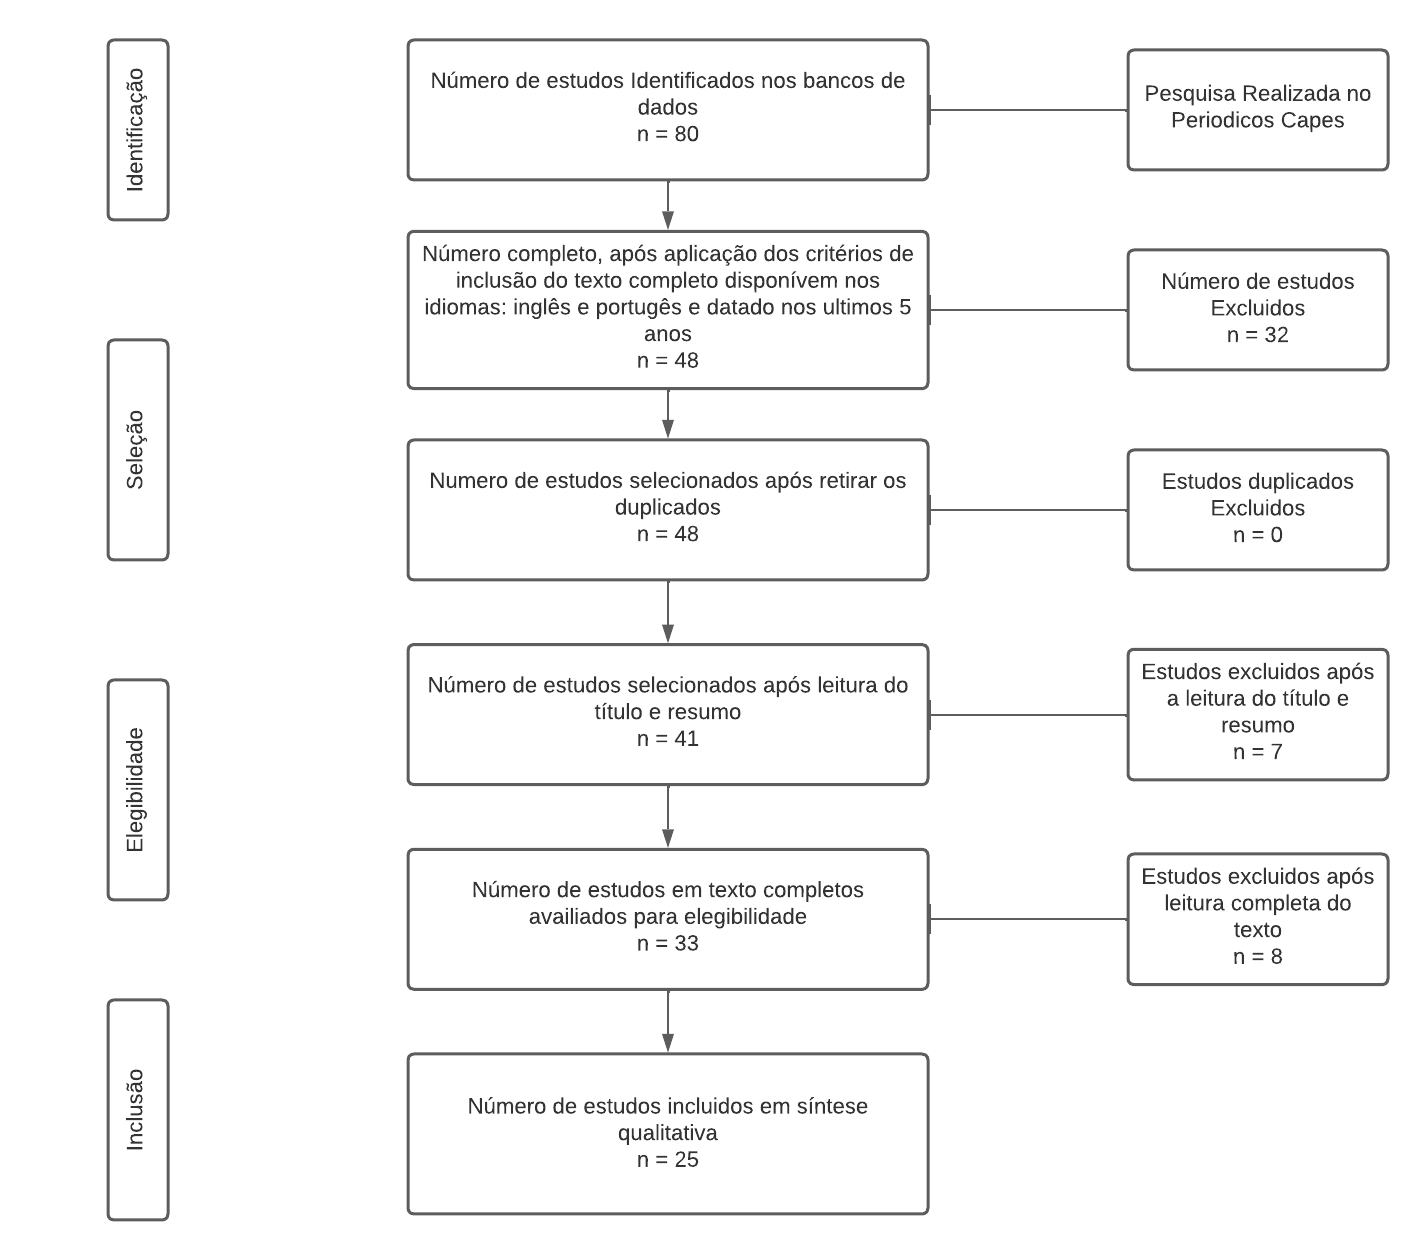
\includegraphics[keepaspectratio=true,scale=0.7]{figuras/Diagrama_Prisma_TCC.png}
	\caption{Diagrama Prisma}
\end{figure}

\section{Metodologia de Desenvolvimento}
\label{md}

Esta seção detalha as especificações da metodologia de desenvolvimento do algorítmo de predição, sendo classificadas em: importação dos dados, pré-processamento, definição do modelo, treino e validação, avaliação, reajustes necessários e previsão, conforme exemplificado na Figura \ref{Fluxo algoritmo}.

\begin{figure}[H]
	\centering
	\label{Fluxo algoritmo}
		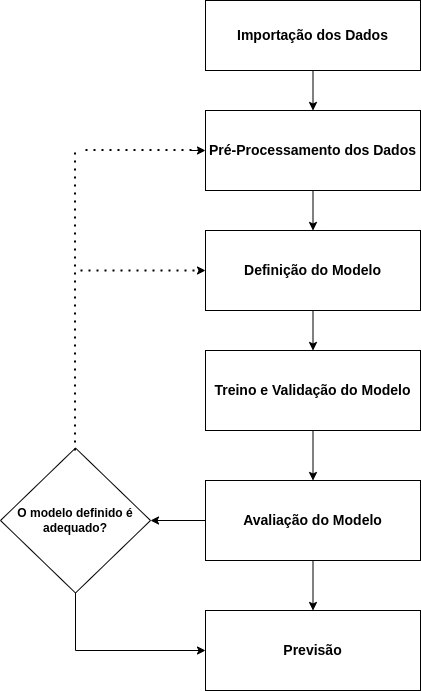
\includegraphics[keepaspectratio=true,scale=0.7]{figuras/diagrama_fluxo_desenv.png}
	\caption{Fluxo de Desenvolvimento do modelo de predição }
\end{figure}

A importação dos dados, consiste na obtenção dos dados históricos do Ibovespa, para realização das análises da série temporal e desenvolvimento das etapas seguintes.

O pré-processamento é realizado para preparar os dados da forma correta, antes de usa-los como entrada no modelo de inteligência artificial para predição do valor da ação.

A etapa de Definição do modelo, será onde iremos definir a arquitetura de rede neural recorrente que será  utilizado e definido os hiperparâmetros explícitos, como o número de épocas e implícitos como o número de camadas, função de ativação e algorítmo de otimização.

No Treino e Validação do Modelo, é realizado o treinamento do modelo com a técnica do \textit{backpropagation}, que usa uma arquitetura hierárquica em camadas de neurônios simples empregando um alto grau de conectividade entre as camadas.\cite{backpropagation} Desta forma, cada nó recebe uma ou mais entradas da camada anterior e produz uma saida que é transmitida para outro nó de entrada da próxima camada. A Equação \ref{backpropag_eq} mostra como é calculado a saída de um determinado nó:

\begin{equation}
\label{backpropag_eq}
    \alpha =  \sum_{i=1}^n  (w_i - x_i) + \theta
\end{equation}

onde {$x_i$} é a entrada no nó, {$w_i$} representa os pesos aplicados as entradas e {$\theta$} é o viés de polarização para o nó e {$n$} é o número de sinapses para o nó.

É esperado uma rede neural totalmente conectada no final quando se utiliza o método \textit{backpropagation}, conforme a Figura \ref{fig_backpropag}.

\begin{figure}[H]
	\centering
	\label{fig_backpropag}
		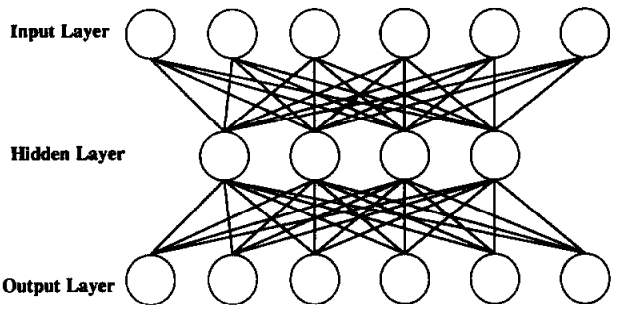
\includegraphics[keepaspectratio=true,scale=0.5]{figuras/backpropag.png}
	\caption{Uma rede de \textit{backpropagation} totalmente conectada \cite{backpropagation}}
\end{figure}

Para a Validação, é realizada o método de \textit{cross-validation}, onde é realizada a comparação de algorítmos de aprendizado dividindo os dados em dois principais segmentos: um é utilizado para para aprender ou treinar o modelo e o outros para validar o modelo, tipicamente, os conjuntos de treinamento e validação devem ser cruzados em rodadas sucessivas, de modo que cada ponto de dados tenha a chance de ser validada. \cite{cross_validation}

Após a etapa de Treinamento e Validação, seguimos para a Avaliação do modelo, onde análisamos as Métricas de Avaliação descritas na Seção \ref{mav} e realizamos todos os possíveis ajustes necessários para que possamos melhorar o modelo até que seja possível de fato temos um resultado relevante para a questão de pesquisa.

Por fim, com o modelo treinado e avaliado, é possível realizar a predição do índice, aplicando o modelo para diversos horizontes temporais.


\section{Metodologia de Análise de Resultados}
\label{mar}

Como citado por \cite{analise_resultados1} além de dominar a metodologia estatística para o planejamento e análise dos dados, o pesquisador deve conhecer bem o que deseja estudar, os dados que irá utilizar e ter uma estimativa qualitativa de como os dados serão analisados.

O físico \cite{analise_resultados2} indica um procedimento para planejamento e análise de resultados em etapas, onde:
 \begin{enumerate}
   \item Reconhecimento e definição do problema que depende da experiência adquirida anteriormente ou do estudo prévio de processos semelhantes
   
   \item Escolha das variáveis e das faixas de valores que as variáveis serão avaliadas. A avaliação de diversas variáveis pode ser necessária quando o estudo encontra-se em seus estágios iniciais, quando deseja-se verificar uma variável específica, o nível de especificação da avaliação dve ser reduzido, além de manter as demais variáveis influentes em níveis constantes.
   
   \item Escolha adequada da variável de resposta, de modo que seja garantido a objetividade na análise dos resultados. A escolha da variável mais adequada se dá mediante ao erro experimental de medida da variável de resposta seja mínimo, permitindo a análise estatística dos dados. 
   
   \item Delineamento dos experimentos: Tamanho da amostra, sequência de execução dos ensaios, necessidade de aleatorização ou uso de blocos. Aprendendo sobre o processo, se deve ser acrescentado novas variáveis ou eliminar variáveis não influentes. Com essa iniciativa, pode-se reduzir o número de ensaios e d
   
   \item Execução dos experimentos, monitorando-os e controlando-os. Etapa que garante a validade experimental, onde exige do pesquisador um conhecimento aprofundado dos métodos de controle e monitoramento aplicados. 
   
   \item Análise dos resultados, com o uso de métodos estatísticos, para que as conclusões estabelecidas sejam objetivas e verdadeiras, garantindo a confiabilidade e a validade dos resultados, de modo que seja possível determinar o erro associado nas conclusões de acordo com o grau de confiança estabelecido.
   
   \item Elaboração das conclusões e recomendações a partir da análise de resultados. Permitirão que decisões sejam tomadas a respeito do processo em estudo, com base em uma documentação, onde pode ser utilizado gráficos e tabelas que apresente de forma clara os resultados obtidos.
   
 \end{enumerate}

\section{Fluxo de Atividades}
\label{fa}

O estudo e execução desse trabalho é orientada por etapas.

A Figura \ref{fluxo_atv} apresenta o fluxograma de atividades seguido, onde é apresentado as etapas e atividades essenciais para a condução desse estudo, contemplando os trabalhos de monografia 1 e 2, e suas apresentações finais respectivas.

\begin{figure}[H]
	\centering
	\label{fluxo_atv}
		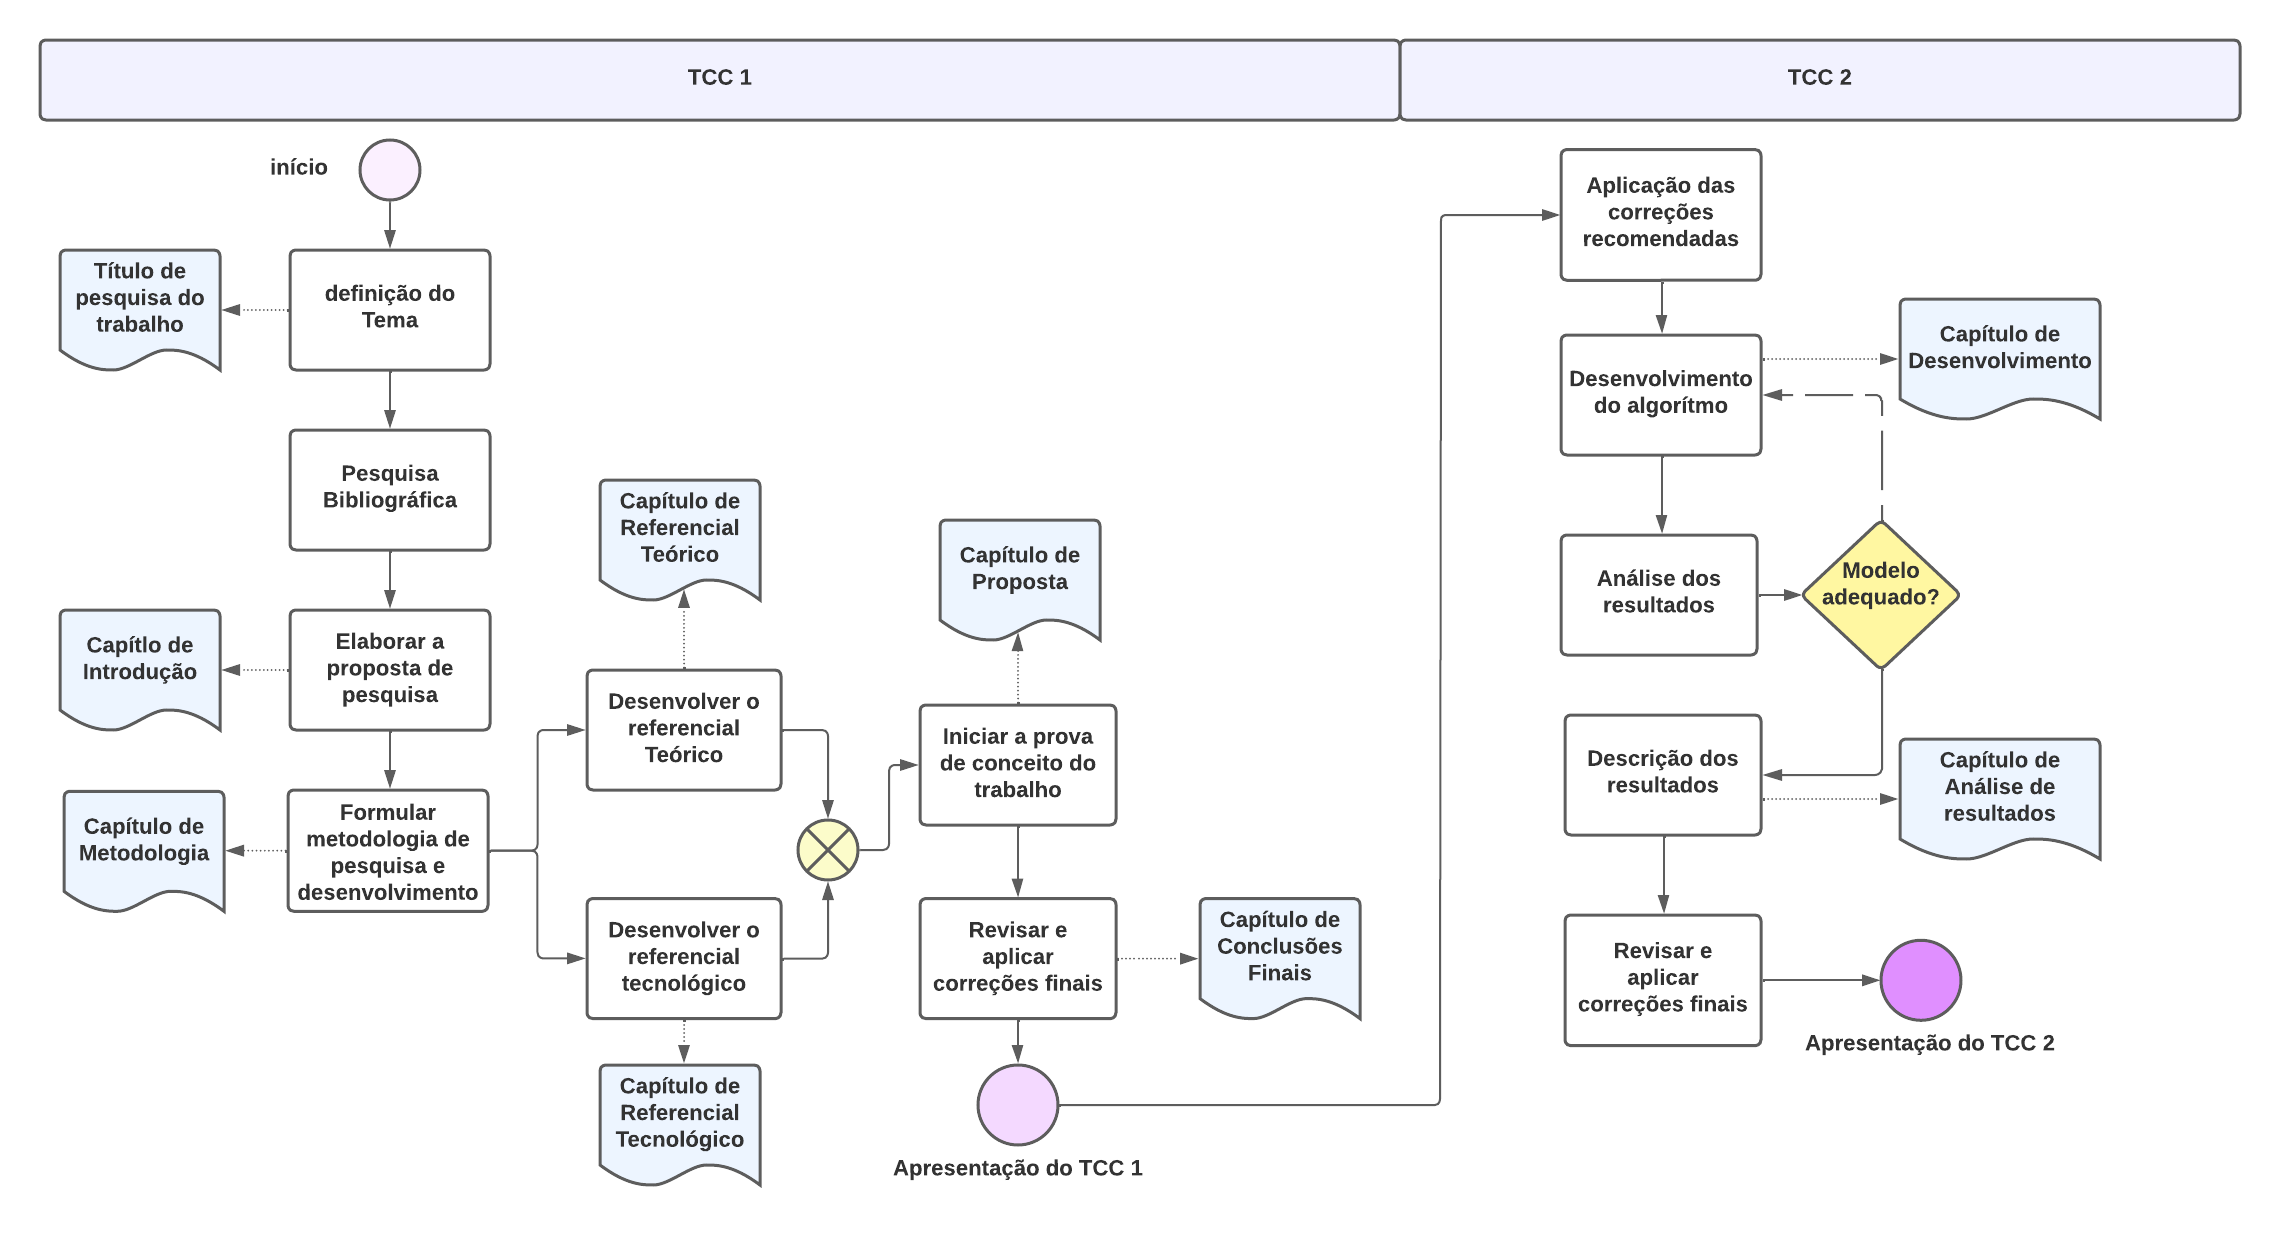
\includegraphics[keepaspectratio=true,scale=0.4]{figuras/fluxo_atv.png}
	\caption{Fluxograma de Atividades da Monografia}
\end{figure}

\textbf{Definição do Tema:} Atividade atribuida a discussão inicial do que o trabalho deveria abordar e refinamento de ideias levantadas através do estudo de redes neurais recorrentes e suas aplicações.

\textbf{Pesquisa Bibliográfica:} Processo de levantamento e coleta de materiais com foco na temática definida, conduzida conforme exemplificado na Seção \nameref{mpi} 

\textbf{Elaboração da proposta de pesquisa:} Etapa que descreve o problema em questão, justificativa, objetivos e contextualização do trabalho proposto.

\textbf{Formulação da metodologia de pesquisa e desenvolvimento:} Atividade que definiu o tipo de pesquisa que este trabalho realizará, com base na abordagem, natureza, objetivos e procedimentos, assim como a especificação da metodologia de desenvolvimento do algorítmo, fluxo de atividades e cronograma de elaboração do trabalho.

\textbf{Desenvolvimento do referencial teórico:} Com base nos principais trabalhos e estudos encontrados em nossa pesquisa bibliográfica, exemplificar os principais conceitos abordados no presente trabalho e com base nas outras pesquisas, entender o que será trabalhado e as métricas que devem ser observadas e relatadas.

\textbf{Desenvolvimento do referencial tecnológico:} Esta atividade expõe todas as principais tecnologias e ferramentas que serão utilizadas na elaboração da pesquisa e desenvolvimento da solução propsota.

\textbf{Inicio da prova de conceito do trabalho:} Esta atividade procura iniciar a proposta de solução, trazendo uma análise inicial do que será abordado futuramente no trabalho de conclusão de curso 2.

\textbf{Revisão e aplicação das correções finais:} Releitura, revisão e aplicação de todas as possíveis correções ao trabalho.

\textbf{Apresentação do TCC 1:} Apresentação a banca julgadora, o trabalho proposto.

\textbf{Aplicação das correções recomendadas:} Após a apresentação, entender as possíveis melhoras e correções apontadas pela banca de forma a termos o melhor trabalho possível.

\textbf{Desenvolvimento do algoríitmo de predição:} Etapa de desenvolvimento da solução proposta inicialmente.

\textbf{Análise e resultados:} Análise dos resultados e comparativo em relação aos principais estudos acerca do tema abordado, conforme descrito da Seção \nameref{mar}.

\textbf{Descrição dos resultados:} Descrição dos principais resultados obtidos e validados à segunda parte da Monografia.

\textbf{Revisão e aplicação das correções finais:} Esta tarefa consiste na revisão de toda a pesquisa e aplicação das ultimas correções necessárias, finalizando as conclusões finais do trabalho realizado.

\textbf{Apresentação do TCC 2:} Apresentação final da segunda e ultima parte da monográfia a banca julgadora.

\section{Cronograma}
\label{crono}

A Tabela \ref{cronograma1} representa o cronograma previsto para as conclusões das tarefas pertencentes ao Trabalho de Conclusão de Curso (TCC) 1, que foi iniciado em Junho de 2022 e tem previsão de conclusão e apresentação ao final do mês de Setembro de 2022. 

\begin{table}[H]
\caption{Cronograma TCC 1}
\label{cronograma1}
\begin{tabular}{@{}llccc@{}}
\toprule
\textbf{\textbf{Atividade}}          & \textbf{Jun/22} & \multicolumn{1}{l}{\textbf{Jul/22}} & \multicolumn{1}{l}{\textbf{Ago/22}} & \multicolumn{1}{l}{\textbf{Set/22}} \\ \midrule
Definição do Tema                    & X               &                                     &                                     &                                     \\ \midrule
Pesquisa Bibliográfica               &                 & X                                   &                                     &                                     \\ \midrule
Introdução                           &                 &                                     & X                                   &                                     \\ \midrule
Referencial Teórico                  &                 &                                     & X                                   &                                     \\ \midrule
Referencial Tecnológico              &                 &                                     & X                                   &                                     \\ \midrule
Metodologia                          &                 &                                     & X                                   &                                     \\ \midrule
Proposta                             &                 &                                     &                                     & X                                   \\ \midrule
Conclusões Finais                    &                 &                                     &                                     & X                                   \\ \midrule
Revisões e finalização da Monografia &                 &                                     &                                     & X                                   \\ \midrule
Apresentação                         &                 &                                     &                                     & X                                   \\ \bottomrule
\end{tabular}
\end{table}

A Tabela \ref{cronograma2} trata as atividades previstas na elaboração do Trabalho de Conclusão de Curso (TCC) 2, que iniciará em Outubro de 2022 e está previsto para finalizar em Fevereiro de 2023.

\begin{table}[H]
\caption{Cronograma TCC 2}
\label{cronograma2}
\begin{tabular}{@{}lccccc@{}}
\toprule
\textbf{Atividade}                       & \multicolumn{1}{l}{\textbf{Out/22}} & \multicolumn{1}{l}{\textbf{Nov/22}} & \multicolumn{1}{l}{\textbf{Dez/22}} & \multicolumn{1}{l}{\textbf{Jan/23}} & \multicolumn{1}{l}{\textbf{Fev/23}} \\ \midrule
Aplicar Correções Sugeridas              & X                                   &                                     &                                     &                                     &                                     \\ \midrule
Análise, limpeza e filtragem dos dados   &                                     & X                                   &                                     &                                     &                                     \\ \midrule
Desenvolvimento do Algorítmo de Predição &                                     &                                     & X                                   &                                     &                                     \\ \midrule
Análise dos Resultados                   &                                     &                                     & X                                   &                                     &                                     \\ \midrule
Otimizações necessárias no modelo        &                                     &                                     &                                     & X                                   &                                     \\ \midrule
Descrição dos Resultados                 &                                     &                                     &                                     & X                                   &                                     \\ \midrule
Finalização da escrita da Monografia     &                                     &                                     &                                     & X                                   &                                     \\ \midrule
Aplicar Correções Necessárias            &                                     &                                     &                                     &                                     & X                                   \\ \midrule
Apresentar                               &                                     &                                     &                                     &                                     & X                                   \\ \bottomrule
\end{tabular}
\end{table}


\section{Considerações Finais}
\label{considfinal}



Este capítulo apresentou os conceitos de pesquisa científica, classificando este estudo quando a abordagem, natureza, objetivos e procedimentos. Definimos a metodologia de pesquisa investigativa, exemplifcando os resultados da construção da \textit{string} de busca e da utilização do guia em diagramação Prisma para obtermos os melhores estudos possíveis correlatos ao tema proposto. Na metodologia de Desenvolvimento, definimos o fluxograma para desenvolvimento do algorítmo de inteligência artificial para perdição do Ibovespa, exemplificando as principais técnicas que são utilizadas no treino e validação do modelo. A metodologia de Análsie de Resultados indica um procedimento para plajenamento de análise de resultados. É apresentado então, o Fluxo de Atividades, onde é listado e exemplificado em ordem de execução e detalhamento cada atividade realizada e a ser realizada para conclusão da monografia. Por fim, tem-se o Cronograma de execução das principais atividades que engloam o Trabalho de conclusão 1 e 2 respectivamente.